\section*{Gendererklärung}

Zur besseren Lesbarkeit werden auf dieser Website personenbezogene Bezeichnungen, die sich zugleich auf Frauen und Männer beziehen, generell nur in der im Deutschen üblichen männlichen Form angeführt, also z.B. \glqq Teilnehmer\grqq{} statt \glqq TeilnehmerInnen\grqq{} oder \glqq Teilnehmerinnen und Teilnehmer\grqq{}.

Dies soll jedoch keinesfalls eine Geschlechterdiskriminierung oder eine Verletzung des Gleichheitsgrundsatzes zum Ausdruck bringen.

\section*{Gender Declaration}

For better readability, personal names that refer to women and men at the same time are generally only given in the masculine form common in German, e.g. \glqq Participants\grqq{} instead of \glqq Participants\grqq{} or \glqq Participants\grqq{}.

However, this is in no way intended to express gender discrimination or a violation of the principle of equality.

\pagebreak

\section*{Eidesstattliche Erklärung}
Hiermit erkläre ich an Eides statt, dass ich die vorgelegte Diplomarbeit selbstständig und ohne Benutzung anderer als der angegebenen Hilfsmittel angefertigt habe. Gedanken, die aus fremden Quellen direkt oder indirekt übernommen wurden, sind als solche gekennzeichnet.

Die Arbeit wurde bisher in gleicher oder ähnlicher Weise keiner anderen Prüfungsbehörde vorgelegt und auch noch nicht veröffentlicht. \\[1em]
Leonding, am \duedatede \\[5em]
\ifthenelse{\isundefined{\firstauthor}}{}{\firstauthor}
\ifthenelse{\isundefined{\secondauthor}}{}{\kern-1ex, \secondauthor}
\ifthenelse{\isundefined{\thirdauthor}}{}{\kern-1ex, \thirdauthor}
\ifthenelse{\isundefined{\fourthauthor}}{}{\kern-1ex, \fourthauthor} \\[5em]

\section*{Declaration of Academic Honesty}
Hereby, I declare that I have composed the presented paper independently on my own and without any other resources than the ones indicated. All thoughts taken directly or indirectly from external sources are properly denoted as such.

This paper has neither been previously submitted to another authority nor has it been published yet. \\[1em]
Leonding, \duedateen \\[5em]
\ifthenelse{\isundefined{\firstauthor}}{}{\firstauthor}
\ifthenelse{\isundefined{\secondauthor}}{}{\kern-1ex, \secondauthor}
\ifthenelse{\isundefined{\thirdauthor}}{}{\kern-1ex, \thirdauthor}
\ifthenelse{\isundefined{\fourthauthor}}{}{\kern-1ex, \fourthauthor} \\[5em]

\begin{abstract}
	An einer Schule sind Klassenräume der wichtigste Ort der Leistunserbringung, die Bedingungen in diesen Klassenräumen sollten für den Lernerfolg optimal sein, in der Realität gibt es oft Mängel (zB sauerstoffarme Luft), die leicht beseitigt werden könnten. Es ist daher Vorteilhaft die Bedingungen in den einzelnen Klassenräumen erfassen zu können, um einerseits Masnahmen zu ergreifen (öffnen der Fenster), andererseits auch um auswertbare Informationen für den Heizbetrieb(Temperatur) zu erhalten.

	Ein Mesh-Netzwerk soll es daher ermöglichen die im gesamten Gebäude der HTL-Leonding verteilten Sensoren und Aktoren zu vernetzen.

	Die Verwendung eines Mesh-Netzwerkes ermöglicht die einfache einbindung von zusätzlichen Sensoren und Aktoren, außerdem wird das Schulnetzwerk nicht beansprucht. 

	Im Rahmen dieser Arbeit wurde zunächst die Mesh-Infrastruktur erstellt (hardwarmäßige Konfiguration und softwaremäßiges Einbinden von Nodes in das Mesh-Netzwerk), weiters wurde als fachliche Anwendung ein IoT-Netzwerk implementiert, welches die Kommunikation zwischen den einzelnen Komponenten mittels eines Message Brokers ermöglicht. Die Visualisierung, als dritte Komponente, kann den aktuellen Zustand des IoT-Netzwerkes dargestellen. Dabei werden folgende Fragen beantwortet: Welche Komponenten (Nodes) sind online, welche Messages (zB Temperaturwerte) werden übermittelt, usw.

	Zusätzlich wurde für die ESP32-Nodes ein Over-The-Air - Update (OTA) implementiert.

	%TODO Bild ändern
	\begin{figure}[H]
        \begin{center}
            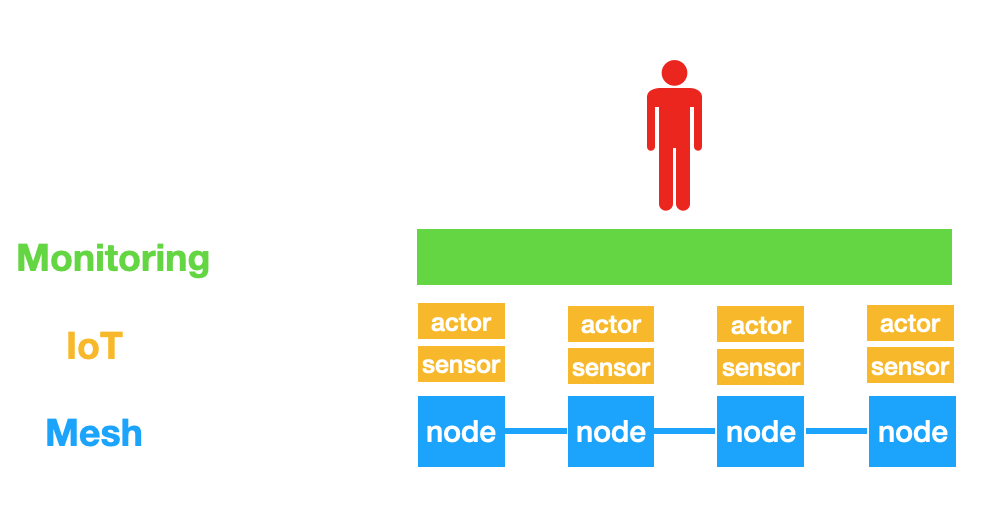
\includegraphics[scale=0.31]{images/structure.png}
            \caption{Struktur (Quelle: eigene Darstellung)}
        \end{center}
    \end{figure}
\end{abstract}

\begin{otherlanguage}{english}
\begin{abstract}
	
	At a school, classrooms are the most important place for the performance of pupils, the conditions in these classrooms should be optimal for learning success, in reality there are often shortcomings (e.g. low-oxygen air) that could easily be remedied. It is therefore advantageous to be able to record the conditions in the individual classrooms in order to take measures (open the window) on the one hand, and to obtain evaluable information for the heating mode (temperature) on the other.

	A mesh network should therefore make it possible to connect the sensors and actuators distributed throughout the HTL-Leonding building.

	The use of a mesh network enables simple integration of additional sensors and actuators, and the school network is not used.

	As part of this work, the mesh infrastructure was initially created (hardware configuration and software integration of nodes into the mesh network), and an IoT network was implemented as an application, which enables communication between the individual components using a message broker. The visualization, as a third component, can represent the current state of the IoT network and answer following questions : Which components (nodes) are online, which messages (e.g. temperature values) are transmitted, etc.

	\begin{figure}[H]
        \begin{center}
            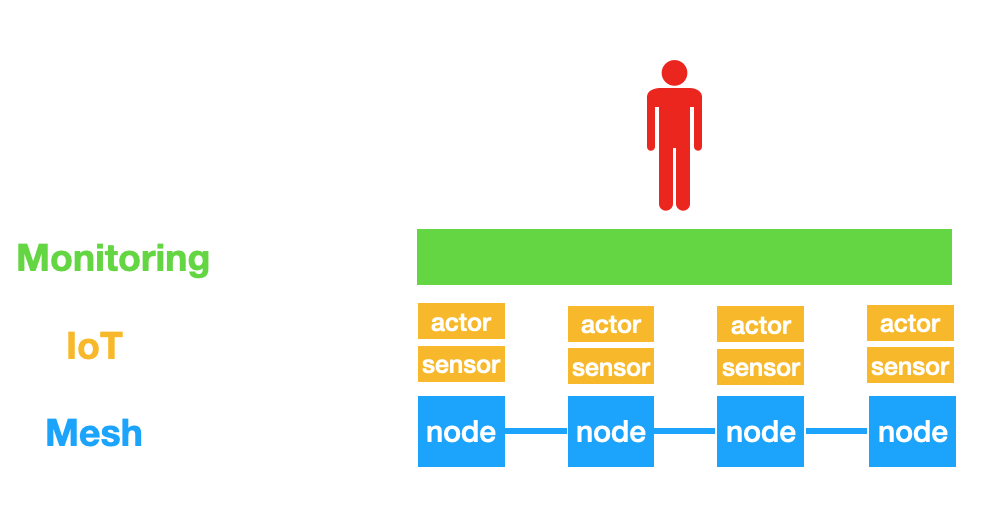
\includegraphics[scale=0.31]{images/structure.png}
            \caption{Structure (source: own source)}
        \end{center}
    \end{figure}
\end{abstract}
\end{otherlanguage}


\section*{Autoren der Diplomarbeit}
\subsection*{Tim Untersberger}
\subsubsection*{Aufgabenbereich}
% TODO: write
\begin{figure}[H]
	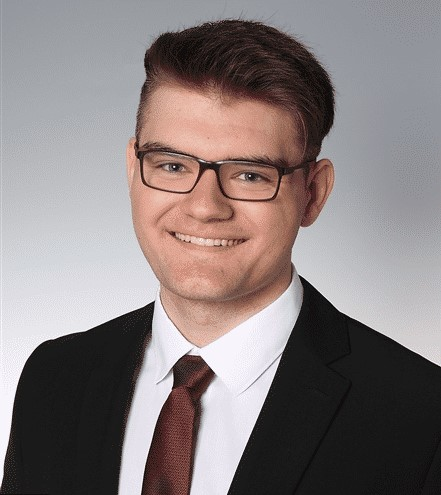
\includegraphics[scale=0.3]{images/tim_untersberger.jpg}
\end{figure}
\begin{table}[htb]
\begin{tabular}{ll}
Name:                            & Tim Untersberger          \\
Geburtsdatum:                    & 15. April 2001                   \\
E-Mail:                          & timuntersberger2@gmail.com          \\
                                 &                               \\
\textbf{Bildungsweg:}            &                               \\  
2007 bis 2011                    & Volksschule Doppl          \\
2011 bis 2015                    & NMS Hart     \\
seit 2015                        & HTL Leonding, Informatik      \\
                                 &                               \\
\textbf{Berufliche Erfahrung:}   &                               \\
Sommer 2016                      & {Colour \& Point}, Softwareentwickler \\
Sommer 2018                      & Runtastic, Softwareentwickler \\
                                 &                               \\
\textbf{Sprachliche Kenntnisse:} &                               \\
Deutsch                          & Muttersprache                 \\
Englisch                         & Fließend                     
\end{tabular}
\caption{Tim Untersberger}
\end{table}
\pagebreak
\subsection*{Stefan Waldl}
\subsubsection*{Aufgabenbereich}
\begin{figure}[H]
	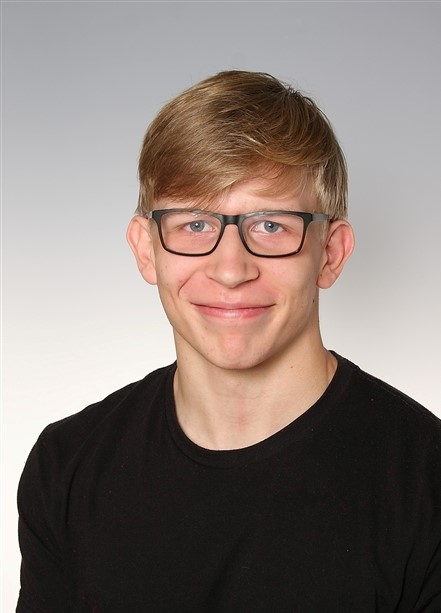
\includegraphics[scale=1]{images/stefan_waldl.jpg}
\end{figure}
\begin{table}[htb]
\begin{tabular}{ll}
Name:                            & Stefan Waldl          		 \\
Geburtsdatum:                    & 26. März 2000                 \\
E-Mail:                          & waldl.stefan@gmail.com        \\
                                 &                               \\
\textbf{Bildungsweg:}            &                               \\  
2006 bis 2010                    & Volksschule 28      		     \\
2010 bis 2015                    & BRG Ramsauerstraße    	 	 \\
seit 2015                        & HTL Leonding, Informatik      \\
                                 &                               \\
\textbf{Berufliche Erfahrung:}   &                               \\
Sommer 2017                      & CBCX-Betting Technologies, Softwareentwickler \\
Sommer 2018                      & CBCX-Betting Technologies, Softwareentwickler \\
                                 &                               \\
\textbf{Sprachliche Kenntnisse:} &                               \\
Deutsch                          & Muttersprache                 \\
Englisch                         & Fließend                     
\end{tabular}
\caption{Stefan Waldl}
\end{table}
\pagebreak
 

\section*{Danksagung}

An dieser Stelle möchten wir uns bei all denjenigen bedanken, die uns während der
Planung und Durchführung dieser Diplomarbeit unterstützt und motiviert haben.

Ganz besonderen Dank an Herrn Prof. Thomas Stütz und Herrn Prof. Gerald Köck, welche uns bereits sehr früh unterstützt und unser Augenmerk auf die richtigen Technologien gelenkt haben, sowie uns auch betreut und unsere Arbeit begutachtet haben.

Bedanken wollen wir uns auch bei all unseren KorrekturleserInnen der Dokumente, welche
uns für eine fehlerfreie und ordentliche Einreichung beiseite standen.